\documentclass[11pt,compress,t,notes=noshow, xcolor=table]{beamer}
\input{../../style/preamble}
\input{../../latex-math/basic-math}
\input{../../latex-math/basic-ml}
\input{../../latex-math/ml-gp}

\newcommand{\titlefigure}{figure_man/discrete/marginalization-more.png} %not best picture
\newcommand{\learninggoals}{
  \item The difference between weight-space and function-space views
}

\title{Advanced Machine Learning}
\date{}

\begin{document}

\lecturechapter{Gaussian Processes: From Weight-space to Function-space}
\lecture{Advanced Machine Learning}


\begin{vbframe}{Weight-Space View}

\begin{itemize}
  \item Until now we considered a hypothesis space $\Hspace$ of parameterized functions $\fxt$ (in particular, the space of linear functions). 
  \item Using Bayesian inference, we derived distributions for $\thetab$ after having observed data $\D$. 
  \item Prior believes about the parameter are expressed via a prior distribution $q(\thetab)$, which is updated according to Bayes' rule 

  $$
  \underbrace{p(\thetab | \Xmat, \yv)}_{\text{posterior}} = \frac{\overbrace{p(\yv | \Xmat, \thetab)}^{\text{likelihood}}\overbrace{q(\thetab)}^{\text{prior}}}{\underbrace{p(\yv|\Xmat)}_{\text{marginal}}}. 
  $$
\end{itemize}

\end{vbframe}


\begin{frame}{Weight-space vs. Function-space View}

\begin{table}
  \begin{tabular}{cc}
  \textbf{Weight-Space View} & \textbf{Function-Space View} \vspace{1mm}\\ 
  Parameterize functions & \\
  \footnotesize Example: $\fxt = \thetab^\top \xv$ & \vspace{1mm}\\
  Define distributions on $\thetab$ & Define distributions on $f$ \vspace{1mm}\\
  Inference in parameter space $\Theta$ & Inference in function space $\Hspace$
  \end{tabular}
\end{table}  


\begin{itemize}
  \item Directly search in a space of \enquote{allowed} functions $\Hspace$.  
  \item Specify a prior distribution \textbf{over functions} instead over a parameter and update it according to the observed data points. 
\end{itemize}


\begin{center}
    
\resizebox{200pt}{80pt}{%




\tikzset{every picture/.style={line width=0.75pt}} %set default line width to 0.75pt        

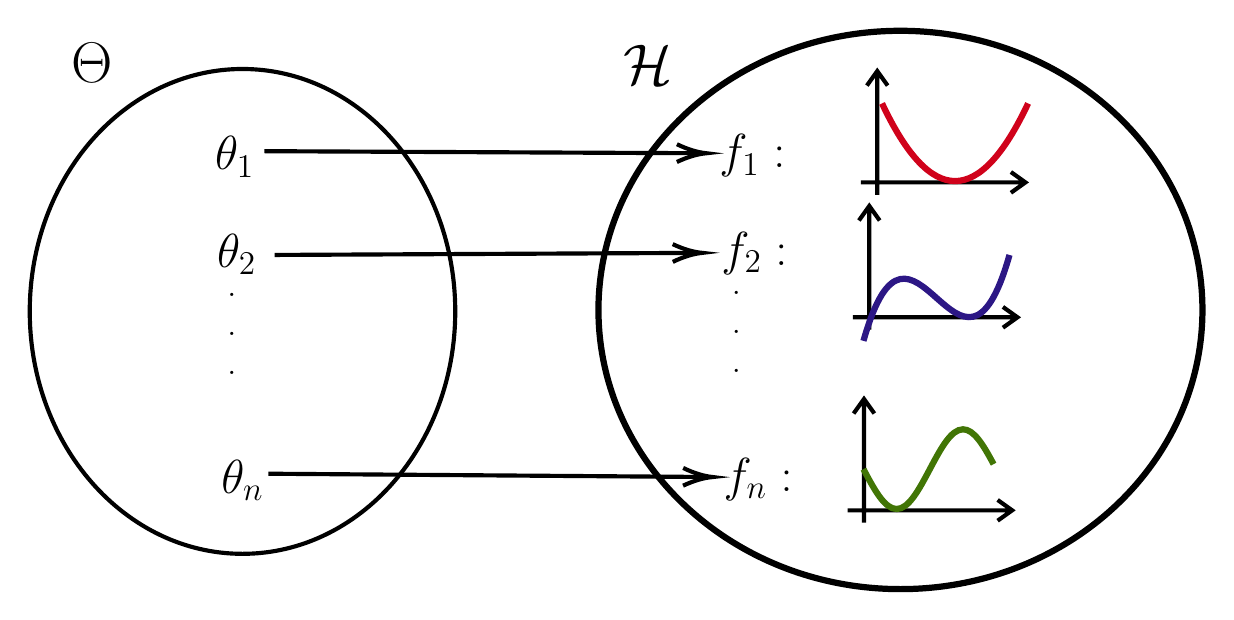
\begin{tikzpicture}[x=0.75pt,y=0.75pt,yscale=-1,xscale=1]
%uncomment if require: \path (0,300); %set diagram left start at 0, and has height of 300

%Shape: Ellipse [id:dp8771691334559413] 
\draw  [line width=1.5]  (48,147.8) .. controls (48,83.29) and (93.89,31) .. (150.5,31) .. controls (207.11,31) and (253,83.29) .. (253,147.8) .. controls (253,212.31) and (207.11,264.6) .. (150.5,264.6) .. controls (93.89,264.6) and (48,212.31) .. (48,147.8) -- cycle ;
%Shape: Ellipse [id:dp5371264326031748] 
\draw  [line width=2.25]  (322,147.1) .. controls (322,72.82) and (387.14,12.6) .. (467.5,12.6) .. controls (547.86,12.6) and (613,72.82) .. (613,147.1) .. controls (613,221.38) and (547.86,281.6) .. (467.5,281.6) .. controls (387.14,281.6) and (322,221.38) .. (322,147.1) -- cycle ;
%Shape: Axis 2D [id:dp35717538747745725] 
\draw [line width=1.5]  (448.4,85.64) -- (527.72,85.64)(456.33,32) -- (456.33,91.6) (520.72,80.64) -- (527.72,85.64) -- (520.72,90.64) (451.33,39) -- (456.33,32) -- (461.33,39)  ;
%Shape: Parabola [id:dp5701843979406445] 
\draw  [color={rgb, 255:red, 208; green, 2; blue, 27 }  ,draw opacity=1 ][line width=2.25]  (458.63,47.6) .. controls (482.09,97.47) and (505.54,97.47) .. (529,47.6) ;
%Shape: Axis 2D [id:dp12458892332319293] 
\draw [line width=1.5]  (444.56,150.64) -- (523.88,150.64)(452.49,97) -- (452.49,156.6) (516.88,145.64) -- (523.88,150.64) -- (516.88,155.64) (447.49,104) -- (452.49,97) -- (457.49,104)  ;
%Shape: Polynomial [id:dp9234268023936685] 
\draw  [color={rgb, 255:red, 44; green, 23; blue, 133 }  ,draw opacity=1 ][line width=2.25]  (449.68,162) .. controls (473.13,79.2) and (496.59,203.4) .. (520.04,120.6) ;
%Shape: Axis 2D [id:dp7374825153612474] 
\draw [line width=1.5]  (442,243.64) -- (521.32,243.64)(449.93,190) -- (449.93,249.6) (514.32,238.64) -- (521.32,243.64) -- (514.32,248.64) (444.93,197) -- (449.93,190) -- (454.93,197)  ;
%Shape: Wave [id:dp7418378470409313] 
\draw  [color={rgb, 255:red, 65; green, 117; blue, 5 }  ,draw opacity=1 ][line width=2.25]  (449.68,223.8) .. controls (454.89,233.64) and (459.88,243) .. (465.67,243) .. controls (471.46,243) and (476.45,233.64) .. (481.66,223.8) .. controls (486.88,213.96) and (491.87,204.6) .. (497.65,204.6) .. controls (502.97,204.6) and (507.61,212.49) .. (512.37,221.39) ;
%Straight Lines [id:da9771831187184936] 
\draw [line width=1.5]    (161,70.6) -- (371,71.59) ;
\draw [shift={(374,71.6)}, rotate = 180.27] [color={rgb, 255:red, 0; green, 0; blue, 0 }  ][line width=1.5]    (14.21,-4.28) .. controls (9.04,-1.82) and (4.3,-0.39) .. (0,0) .. controls (4.3,0.39) and (9.04,1.82) .. (14.21,4.28)   ;
%Straight Lines [id:da20841612893286743] 
\draw [line width=1.5]    (166,120.6) -- (369,119.61) ;
\draw [shift={(372,119.6)}, rotate = 179.72] [color={rgb, 255:red, 0; green, 0; blue, 0 }  ][line width=1.5]    (14.21,-4.28) .. controls (9.04,-1.82) and (4.3,-0.39) .. (0,0) .. controls (4.3,0.39) and (9.04,1.82) .. (14.21,4.28)   ;
%Straight Lines [id:da00018388206135444563] 
\draw [line width=1.5]    (163,226) -- (374,227.58) ;
\draw [shift={(377,227.6)}, rotate = 180.43] [color={rgb, 255:red, 0; green, 0; blue, 0 }  ][line width=1.5]    (14.21,-4.28) .. controls (9.04,-1.82) and (4.3,-0.39) .. (0,0) .. controls (4.3,0.39) and (9.04,1.82) .. (14.21,4.28)   ;

% Text Node
\draw (136,62.4) node [anchor=north west][inner sep=0.75pt]  [font=\LARGE]  {$\boldsymbol{\theta }_{1}$};
% Text Node
\draw (137,109.4) node [anchor=north west][inner sep=0.75pt]  [font=\LARGE]  {$\boldsymbol{\theta }_{2}$};
% Text Node
\draw (139,218.4) node [anchor=north west][inner sep=0.75pt]  [font=\LARGE]  {$\boldsymbol{\theta }_{n}$};
% Text Node
\draw (142,138) node [anchor=north west][inner sep=0.75pt]  [font=\large] [align=left] {.\\.\\.};
% Text Node
\draw (379,61.4) node [anchor=north west][inner sep=0.75pt]  [font=\LARGE]  {$f_{1} :$};
% Text Node
\draw (380,108.4) node [anchor=north west][inner sep=0.75pt]  [font=\LARGE]  {$f_{2} :$};
% Text Node
\draw (381,217.4) node [anchor=north west][inner sep=0.75pt]  [font=\LARGE]  {$f_{n} :$};
% Text Node
\draw (385,137) node [anchor=north west][inner sep=0.75pt]  [font=\large] [align=left] {.\\.\\.};
% Text Node
\draw (333,18.4) node [anchor=north west][inner sep=0.75pt]  [font=\huge]  {$\mathcal{H}$};
% Text Node
\draw (67,17.4) node [anchor=north west][inner sep=0.75pt]  [font=\huge]  {$\Theta $};


\end{tikzpicture}





}

\end{center}

\end{frame}

\begin{vbframe}{Function-space View}

Intuitively, imagine we could draw a huge number of functions from some prior distribution over functions $^{(*)}$. 

\begin{figure}
  \includegraphics[width=0.8\textwidth]{figure/gp_sample/1_1.pdf}
\end{figure}

\vspace*{-0.5cm}

\begin{footnotesize}
  $^{(*)}$ We will see in a minute how distributions over functions can be specified. 
\end{footnotesize}

\end{vbframe}

\begin{frame}{Function-space View}

    After observing some data points, we are only allowed to sample those functions, that are consistent with the data. \\

  \begin{figure}
\foreach \x in{1,2,3} {
    \includegraphics<\x>[width=0.8\textwidth]{figure/gp_sample/2_\x.pdf}\par
    }
  \end{figure}

\end{frame}

\begin{vbframe}{Function-space View}

As we observe more and more data points, the variety of functions consistent with the data shrinks. 
  \begin{figure}
    \includegraphics[width=0.8\textwidth]{figure/gp_sample/2_4.pdf}
  \end{figure}

\framebreak 

Intuitively, there is something like \enquote{mean} and a \enquote{variance} of a distribution over functions. 

  \begin{figure}
    \includegraphics[width=0.8\textwidth]{figure/gp_sample/2_4.pdf}
  \end{figure}

\end{vbframe}






\endlecture
\end{document}
